\graphicspath{
    {figures_and_references/urban_surface_detection/}
    {figures_and_references/EELISA_conference/}
}

% \selectlanguage{english}
\renewcommand{\chapternametext}{Chapter \thechapter: Aerial imagery and image vision}

\begin{refsection}

\chapter{\chapternametext}
\

\renewcommand{\headingtextL}{}
\renewcommand{\headingtextR}{\chapternametext}

\begingroup
 \flushbottom
 \setlength{\parskip}{0pt plus 1fil}%
 \localtableofcontents 
\endgroup

\begingroup
 \flushbottom
 \setlength{\parskip}{0pt plus 1fil}%
 \locallistoffigures
\endgroup


\newpage

\setcounter{section}{0} 



\FloatBarrier

\renewcommand{\sectionnametext}{Introduction}
\renewcommand{\headingtextL}{\chapternametext}
\renewcommand{\headingtextR}{\thesection. \sectionnametext}
\section{\sectionnametext}

Satellite imagery has been globally accessible for the past two decades, while high-resolution aerial imagery from airplanes has been available since the mid-20th century. Both current and historical images are freely accessible for research via services like Google Earth Engine \footcite{gorelick_google_2017} and national or local cartography providers. 

Vectorial cartography is created by tracing aerial imagery. OpenStreetMap (OSM), the largest crowd-sourced project, relies on this method for global vectorial cartography \footcite{haklay_openstreetmap_2008}. However, this manual process is labor-intensive, resulting in incomplete data, especially in non-common categories like on-street parking spaces. Historical urban analysis is challenging due to scarce, less detailed historical cartography. \\


Aerial imagery is widely available, but vectorial cartography data is more accessible in developed regions with Spatial Data Infrastructures (SDIs) like the European Union’s INSPIRE scheme, which standardizes geospatial datasets \footcite{noauthor_directive_2007, minghini_comparing_2019}. However, categories may lack clear definitions. For instance, parking falls under RoadService without further subdivisions. 
In major European cities, openly accessible vector cartography following the INSPIRE scheme usually undergo  
annual updates \footcite{noauthor_city_nodate, noauthor_stadtvermessung_nodate,
paris_city_council_paris_nodate, 
noauthor_luftbilder_nodate, 
ayuntamiento_de_madrid_geoportal_nodate}. 

OSM, as it is maintained by volunteers, does not follow the INSPIRE scheme but offers diverse geospatial data based on local needs \footcite{minghini_comparing_2019}. OSM enables collaboration for rapid cartography, especially useful for humanitarian mapping post-disasters \footcite{herfort_evolution_2021}. OSM has 88931 
different keys, but the dataset is not comprehensive, and the absence 
of numerous objects can be anticipated. The data's quality varies, posing challenges for scientific studies \footcite{minghini_openstreetmap_2019, haklay_how_2010}. \\


Classical and machine learning-enhanced remote sensing methods utilizing multispectral imagery \footcite{sharifi_application_2020,sharifi_nitrogen_2022,nejad_multispectral_2023,esmaeili_hyperspectral_2023,jalayer_assessment_2023} are insufficient for identifying parking surfaces. These techniques primarily classify surface materials, textures, and patterns, which often make parking areas indistinguishable from roads. Since parking spaces are typically inferred through additional contextual information, a specialized machine learning approach is necessary. This approach should focus on features such as road markings, texture variations, vehicle positions, and other contextual indicators. Another advantage of utilizing optical imagery and machine learning is the availability of high-quality imagery within the optical spectrum. 


Advancements in computer vision and object detection \footcite{zou_object_2023} have enabled significant progress in semantic segmentation and object detection for aerial imagery, benefiting a wide range of fields \footcite{yuan_review_2021}. Until recently, vision models were predominantly based on convolutional neural networks and were trained for specific tasks using topic-specific datasets with a fixed number of classes \footcite{thisanke_semantic_2023, mauricio_comparing_2023}. The limitations of these models included their difficulty in handling images significantly different from the training context, an issue that domain adaptation techniques sought to address \footcite{singhal_domain_2023}, as well as their inflexibility in labeling schemes, where introducing new labels was not straightforward.


In contrast, recent transformer-based vision models, known as foundational models \footcite{awais_foundational_2023}, are trained on extensive and diverse datasets sourced from the internet. These models can perform a broad range of tasks, such as general object segmentation, across various types of images. Models such as SAM \footcite{kirillov_segment_2023} incorporate text-processing capabilities to interpret image labels and are designed to handle an unfixed number of classes. Moreover, they can potentially identify new labels without additional training, provided these labels are sufficiently similar to those in the training dataset.


However, these models often lack precision when applied to tasks that differ significantly from their training data, such as analyzing aerial imagery or segmenting uncommon elements like parking surfaces. With the increasing availability of high-resolution aerial imagery and detailed cartography, it is essential to establish automated workflows for creating specialized training datasets using open data and developing fine-tuning methodologies to adapt foundational models for specific tasks and diverse environments. Fine-tuning transformer-based vision models has already been explored in other contexts \footcite{sandler_fine-tuning_2022}.\\ 

\renewcommand{\sectionnametext}{Aerial imagery}
\renewcommand{\headingtextR}{\thesection. \sectionnametext}
\section{\sectionnametext}

Aerial optical imagery is globally accessible. Satellites provide lower-resolution images, with NASA's Landsat 8 and 9 offering 15-meter resolution and an 8-day revisit time \footcite{noauthor_usgs_nodate}, and ESA's Sentinel 2 providing 10-meter resolution with a 5-day revisit time \footcite{noauthor_copernicus_nodate}. Both agencies offer WMTS services for true-color images covering the entire Earth. Private companies like DigitalGlobe provide higher-resolution imagery (up to 30 cm), but access is limited and requires payment \footcite{digitalglobe_worldview-3_nodate}. High-resolution satellite imagery, is therefore available in significant portions of the world. While sufficient for building footprint geometry extraction, distortions and variations in brightness and contrast, along with shadows, can compromise accuracy and orthorectification is less effective, making gaps less visible when determining whether two structures are isolated or touching or for more detailed applications.

Drone or airplane images offer higher resolutions, typically 20 to 5 cm per pixel. For instance segmentation and detailed semantic segmentation, resolutions finer than 1 meter are often needed [fig \ref{fig:image_res
}]. 

\begin{figure}[!htp]
\centering
\begin{tabular}{cc}
\begin{subfigure}[t]{0.45\linewidth}
\centering
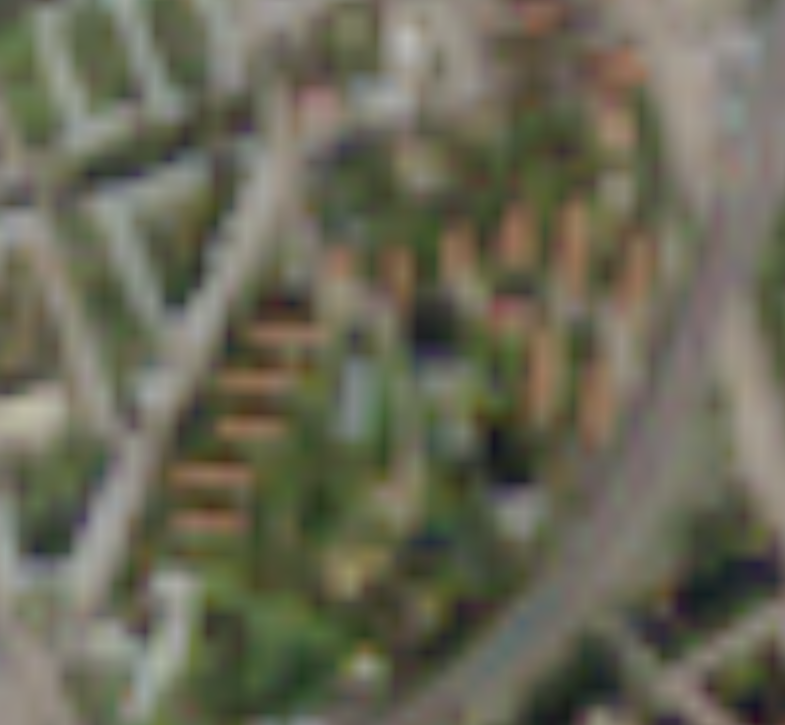
\includegraphics[width=4.5cm, height=3cm]{figures/fig_sentinel2.png}
\caption{Sentinel 2 10 m resolution image in Vienna (Source: Copernincus).}
\label{fig:vienna_10m
}
\end{subfigure} &
\begin{subfigure}[t]{0.45\linewidth}
\centering
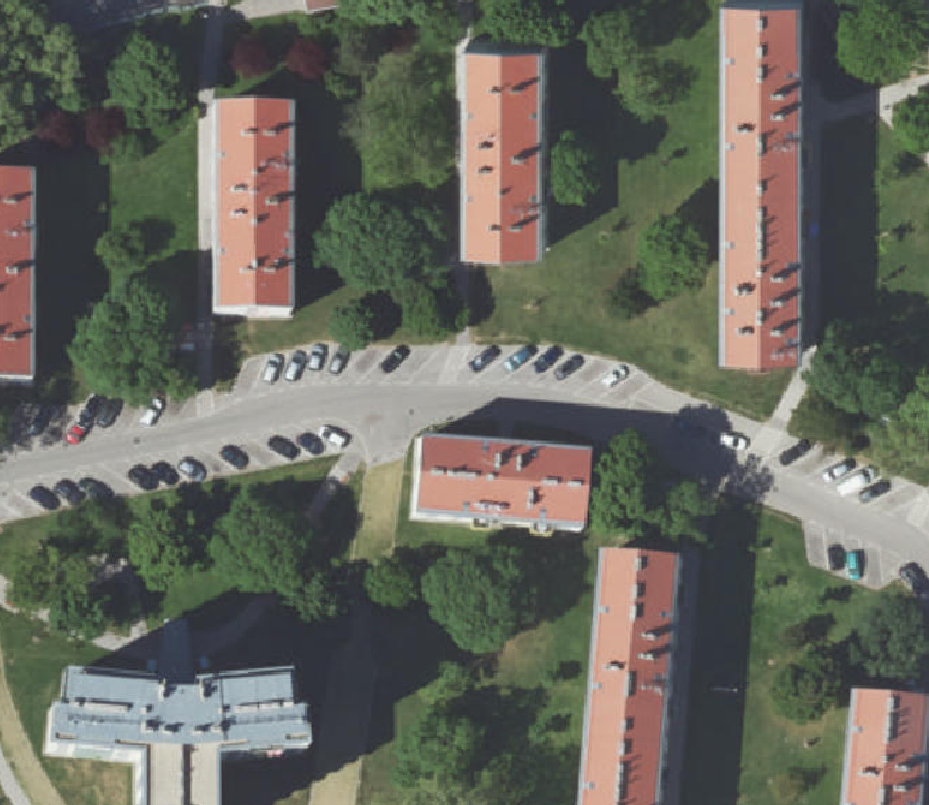
\includegraphics[width=4.5cm, height=3cm]{figures/fig_wienlb.png}
\caption{20 cm resolution orthophoto in the same area (Source: Geoportal of the City of Vienna).}
\label{fig:vienna_20_cm
}
\end{subfigure}
\end{tabular}
\caption{The importance of image resolution.}
\label{fig:image_res
}
\end{figure}

Google Earth \footcite{noauthor_google_nodate} offers global aerial photography with resolutions from 15 meters to 10 cm. However, controlling the date and quality of images is challenging due to stitching from multiple sources. 

European cities provide public vector cartography and orthophotography with resolutions of 20 to 5 cm, updated annually \footcite{noauthor_city_nodate, noauthor_stadtvermessung_nodate, paris_city_council_paris_nodate, noauthor_luftbilder_nodate, ayuntamiento_de_madrid_geoportal_nodate}. These datasets are available via cloud services following Open Geospatial Consortium standards \footcite{maidment_open_2011}. Historic aerial images since 1950 are often available. Overall, sufficient resolution imagery is available in most regions.

Aerial imagery is inherently subject to distortions caused by camera tilt and terrain topography. Orthorectification techniques mitigate these distortions, enabling precise measurements. This is particularly crucial in urban environments. Ineffective orthorectification can obscure gaps between buildings, reducing accuracy when assessing whether structures are isolated or touching. Furthermore, the visibility of building facades, which can be easily confused with roofs, frequently results in footprints appearing larger than their actual dimensions.
(fig. \ref{fig:distortion}).

\begin{figure}[!htp]
\centering
\begin{tabular}{ccc}
\begin{subfigure}[t]{0.3\linewidth}
\centering
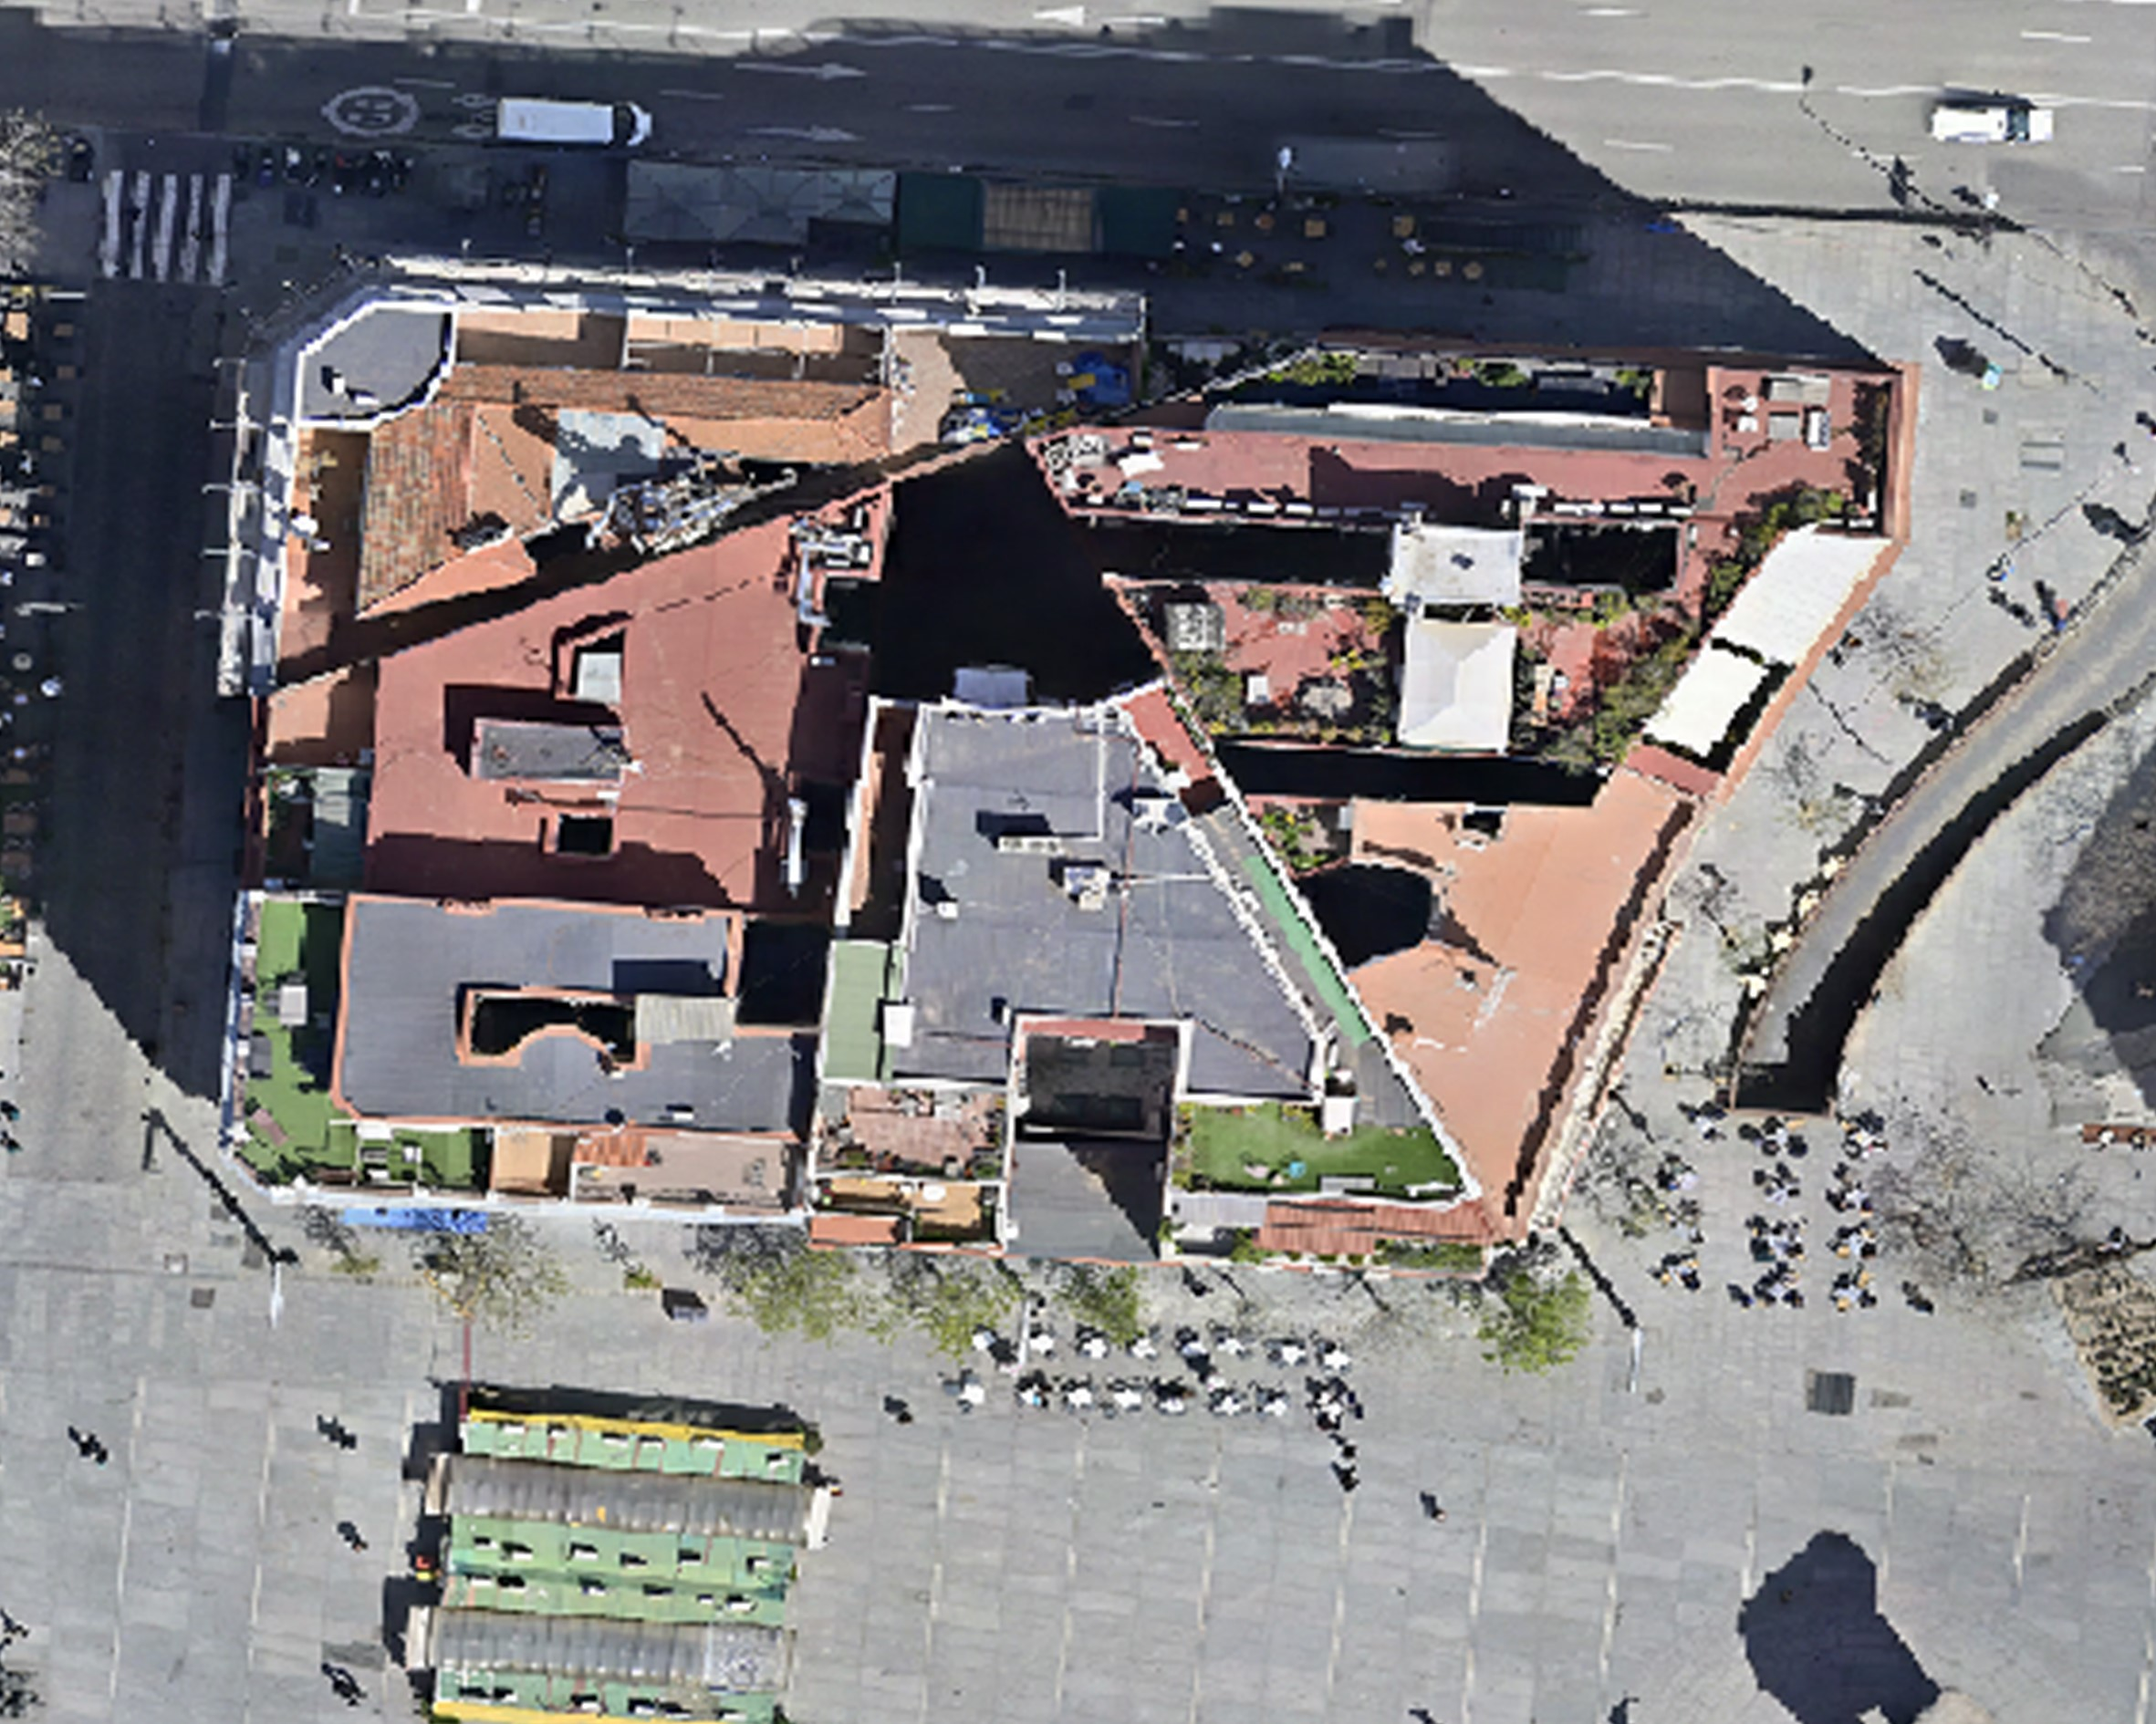
\includegraphics[width=4cm, height=3cm]{figures/wizink_1_5.JPG}
\caption{1.5 cm/pix UAV image.}
\label{fig:1.5cma
}
\end{subfigure}
&
\begin{subfigure}[t]{0.3\linewidth}
\centering
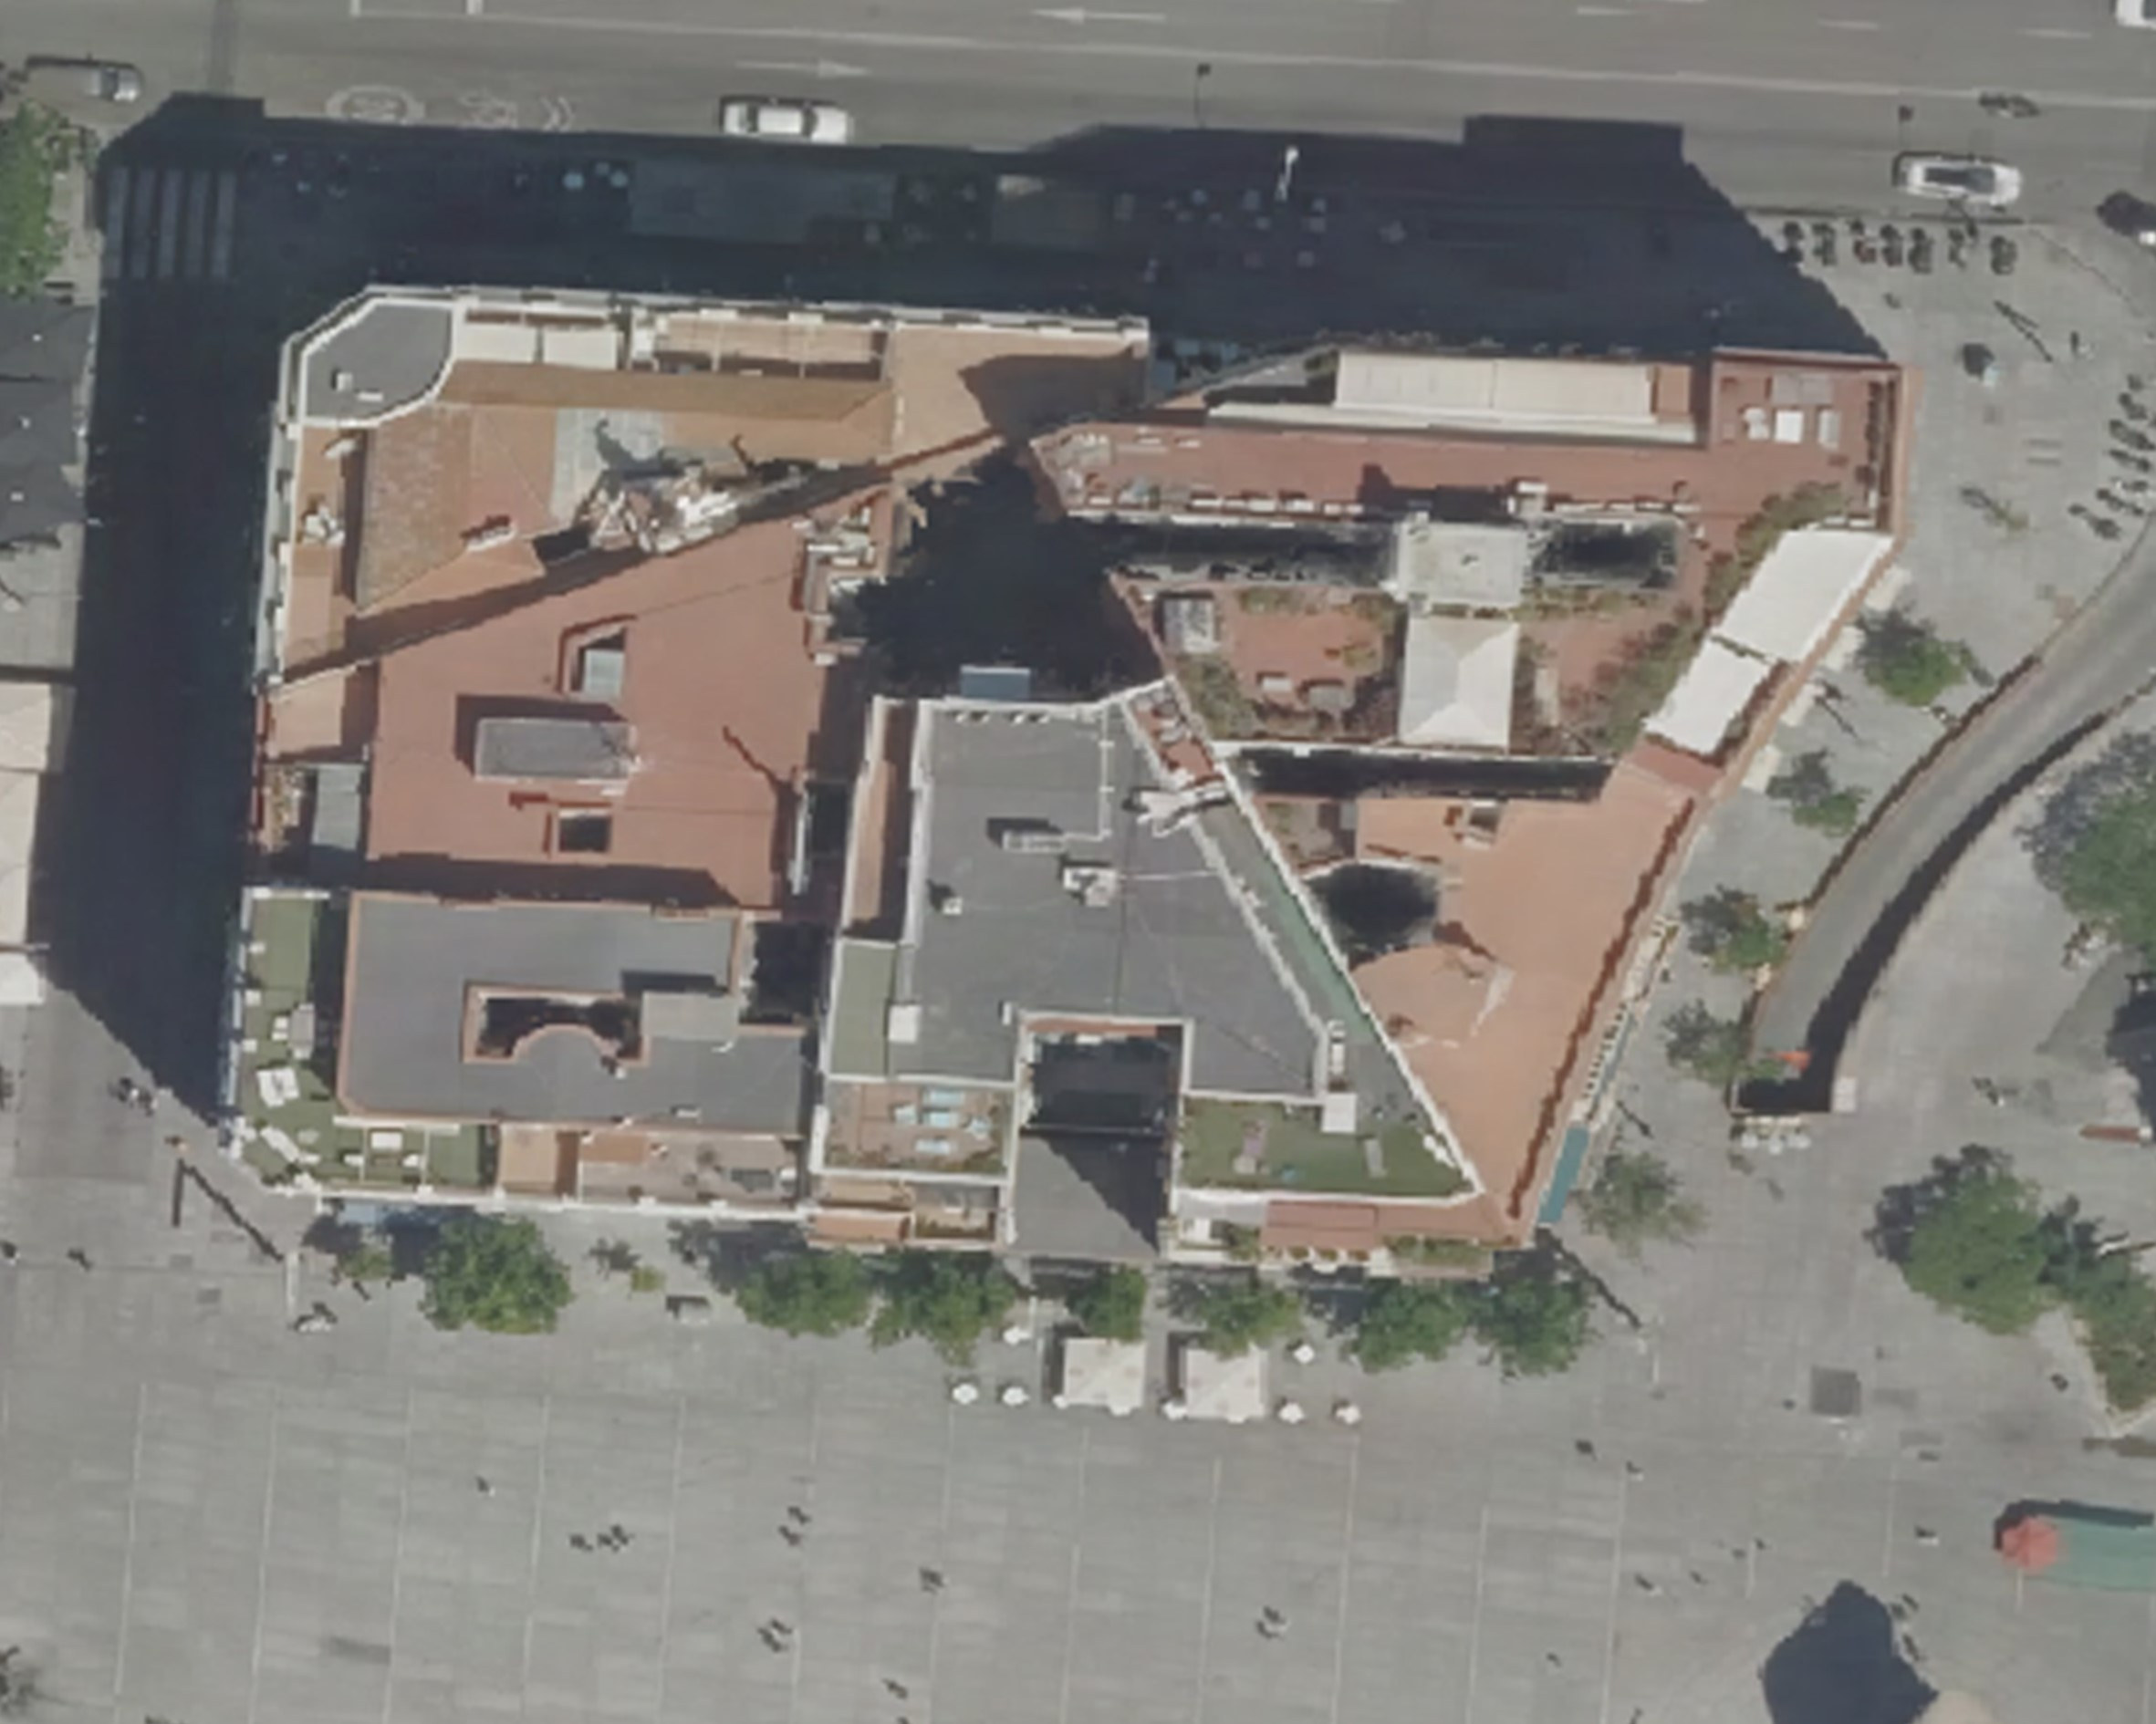
\includegraphics[width=4cm, height=3cm]{figures/wizink_10.JPG}
\caption{10 cm/pix Aerial image.}
\label{fig:10cmb
}
\end{subfigure}
&
\begin{subfigure}[t]{0.3\linewidth}
\centering
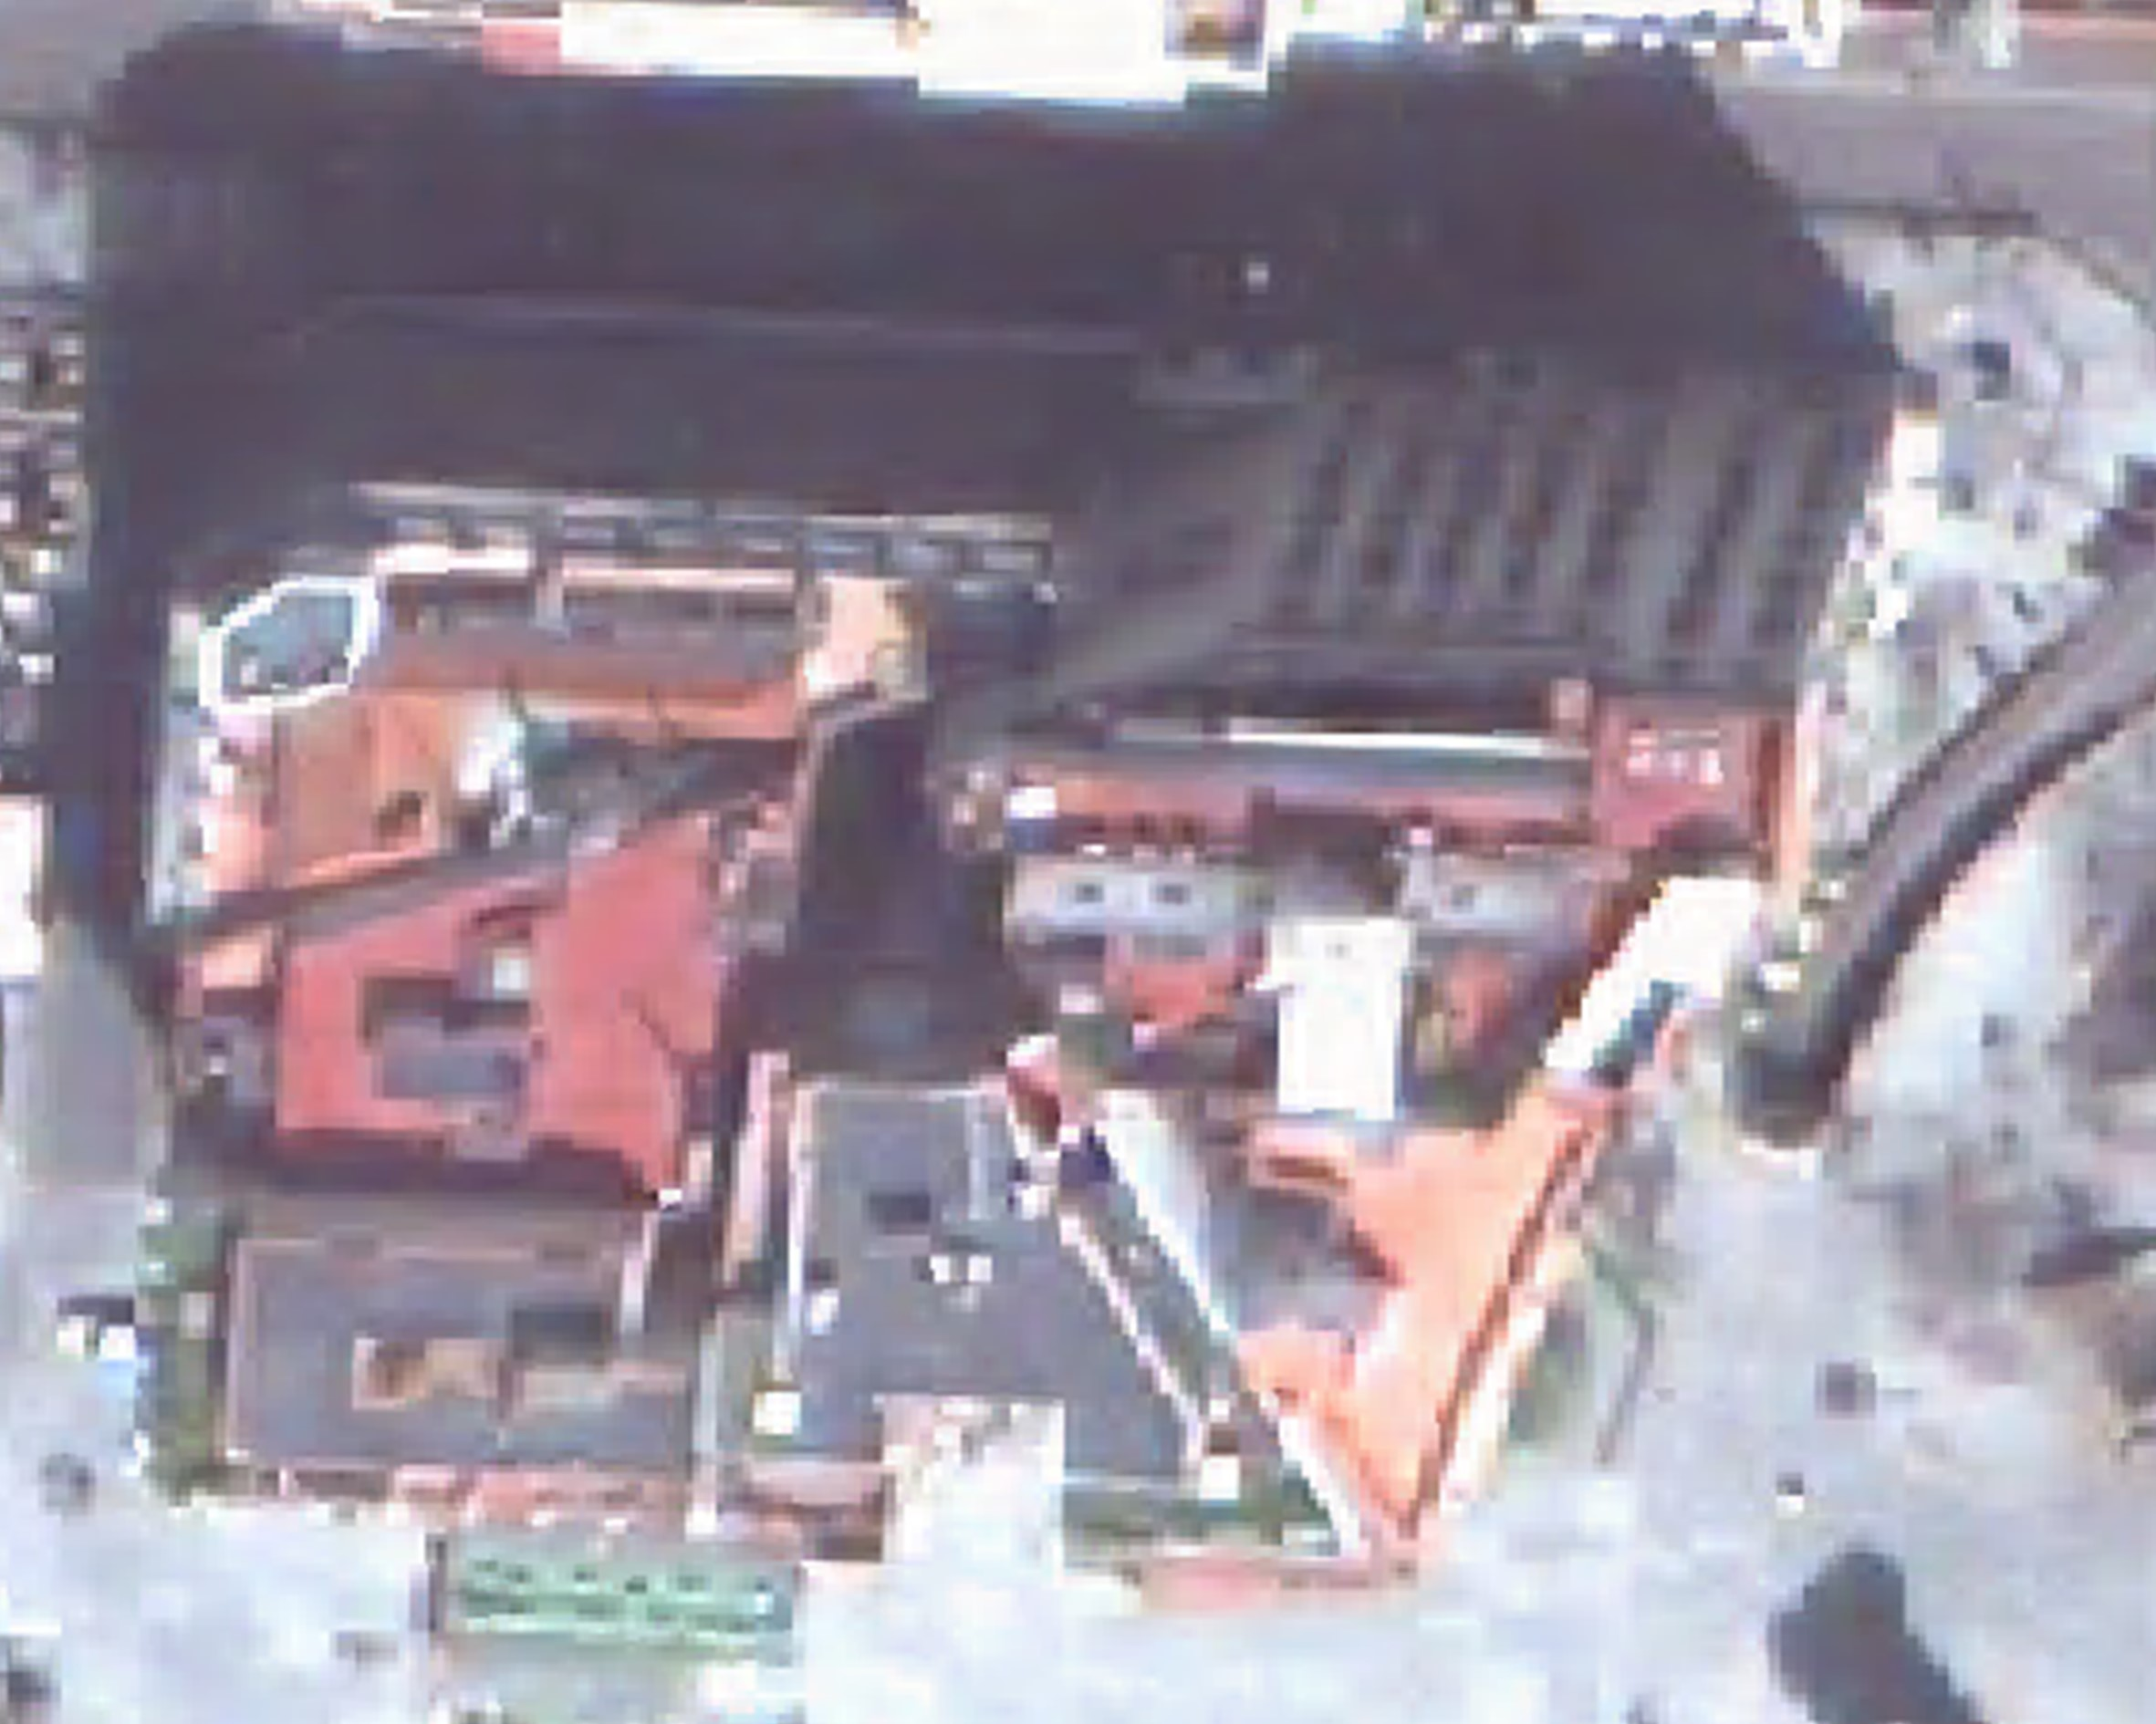
\includegraphics[width=4cm, height=3cm]{figures/wizink_30.JPG}
\caption{30 cm/pix Satellite (WorldView3) image.}
\label{fig:30cmc
}
\end{subfigure}
\end{tabular}
\caption{Remaining distortion in orthoimages of a building in Madrid taken by UAV (least distortion), plane, and satellite (most distortion) (Source: Ayuntamiento de Madrid, 2023).}
\label{fig:distortion}
\end{figure}

\renewcommand{\sectionnametext}{Image vision}
\renewcommand{\headingtextR}{\thesection. \sectionnametext}
\section{\sectionnametext}

Machine learning has seen extensive application in remote sensing 
and object detection over the last decade 
\footcite{zou_object_2023}. 
In the earlier stages, 
traditional statistical methods were prevalent for tasks 
like automatic road extraction \footcite{mena_state_2003}. 
However, machine learning methods have surpassed traditional approaches 
in recent years \footcite{zou_object_2023}. Various datasets and benchmarks for semantic segmentation 
tasks related to building detection, land use and cover extraction, 
and road geometry are available \footcite{zamir_isaid_2019,
helber_introducing_2018, 
mnih_machine_2013, 
marmanis_semantic_2016}.


Machine learning models working with aerial imagery in the optical spectrum have been developed for diverse applications, including land use detection \footcite{talukdar_land-use_2020, nasiri_land_2022}, building detection \footcite{zhu_map-net_2021, dong_review_2024, shao_brrnet_2020, liu_building_2019}, urban mapping \footcite{mohammadi_evaluation_2021}, road geometry extraction \footcite{mattyus_deeproadmapper_2017, zhang_road_2018}. 


In most cases, these machine learning models are based on image 
convolutions. They play a vital role in annotating maps 
\footcite{jiao_machine_2018, 
abdurakhmonov_advances_2023} and exhibit high 
accuracy when tested in environments similar to the training data, 
but a low generability to unknown environments. 
Additionally, machine learning models can be utilized to correct 
OpenStreetMap (OSM) data 
\footcite{vargas-munoz_openstreetmap_2021}.


Researchers have explored the labeling and creation of more diverse  
datasets to enhance the generability of aerial imagery 
segmentation models across diverse global environments 
\footcite{maggiori_can_2017}. However, addressing 
this challenge remains an ongoing effort. Recent advancements include 
the development of general purpose models that leverage 
transformer-based machine learning architectures for geospatial 
analysis \footcite{wu_samgeo_2023}. 
A commercially available 
plugin for QGIS is now accessible 
\footcite{aszkowski_deepness_2023} to run such models 
directly.


Datasets like GBSS 
\footcite{hu_gbssglobal_2024} by Google and 
ML Building Footprints by Microsoft 
\footcite{microsoft_globalmlbuildingfootprints_2024} provide 
building footprints worldwide. Both datasets where 
created with machine learning models trained with OSM data. 
The datasets may not have a very high quality  
\footcite{gonzales_building-level_2023}, especially 
when precise annotations are required or when models are tested in 
regions outside the Western world. \\

\subsection{Semantic segmentation}

Semantic segmentation consist in assigning a label to each pixel of an image. The output are raster values and the technique is not suitable for producing vectorial geometries. The most widely used deep learning models for image segmentation,
fully convolutional neural networks \footcite{long_fully_2015},
employ image convolutions where the parameters of the kernel
are training parameters. Semantic segmentation models usually follow a 
encoder-decoder structure \footcite{badrinarayanan_segnet_2016}. \\ 


Until recently fully convolutional neural networks where the standard for
semantic segmentation tasks. Recently language related tasks with deep
learning saw a large improvement with transformer based models
\footcite{vaswani_attention_2023}. For image related tasks a vision transformer
was developed \footcite{dosovitskiy_image_2020} and powerful universal models became available, such as Mask2Former \footcite{cheng_masked-attention_2022}.


The availability of large datasets combined with the computational power of transformer models has led to a new trend: the development of foundational models \footcite{awais_foundational_2023}. These are models trained on massive datasets using computational resources typically accessible only to the largest technology companies, designed for general or multi-purpose tasks. Two notable examples of foundational models in the field of image vision are the DaTaSeg model \footcite{gu_dataseg_2023} and the Segment Anything Model (SAM) \footcite{kirillov_segment_2023}. These models enable automatic segmentation of objects and instances, without being tied to a specific topic or dataset. They also facilitate the creation of semi-supervised and coarsely annotated datasets. The SAM model includes a GPT module 
allowing any user to input an image and a text prompt. The model segments the image
according to the text given by the user (one shot segmentation). Another option provided by the 
model is to segment unknown objects in the image without providing any 
prompt or additional training (zero shot segmentation). 
A geospatial version 
SAM is available \footcite{wu_samgeo_2023} through the 
SamGeo python package but employing the same trained model. The training dataset, the SA-1B dataset,  
comprises general images sourced from the internet \footcite{kirillov_segment_2023} 
using information such as alt texts to train text promts, 
while the application involves aerial images, which possess markedly 
distinct characteristics and segmentation classes 
compared to the training data. 
General purpose semantic segmentation models such as 
SAM are effective in the context of geospatial 
analysis for general and easy tasks as segmenting buildings 
or detecting forests \footcite{osco_segment_2023}, 
but for a specific
task like detecting parking spaces it fails completely (fig. \ref{fig:SAM}). \\

\begin{figure}[H]
    \centering
    \begin{tabular}{cc}
        \subcaptionbox{SAM model results when segmenting building roofs.}{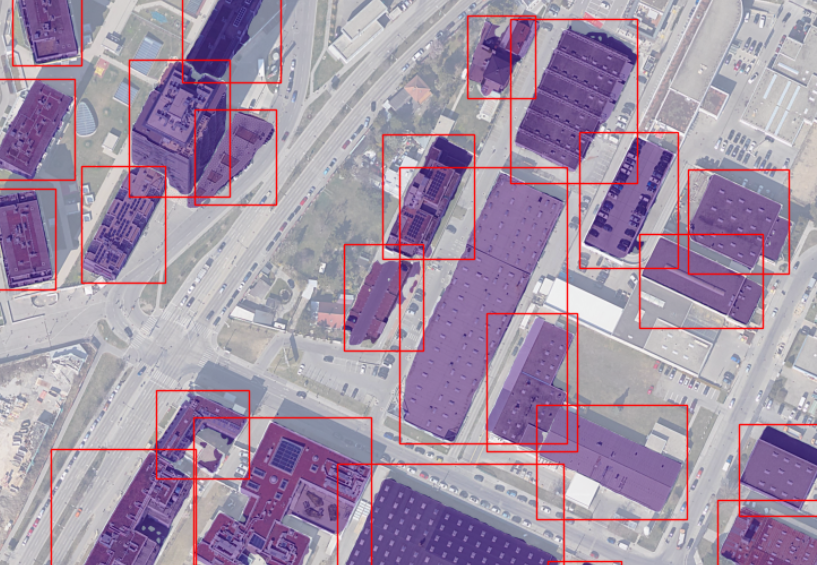
\includegraphics[width=5cm,height=3cm]{figures/fig_SAM_building.png}} &
        \subcaptionbox{SAM model results when segmenting parking spaces.}{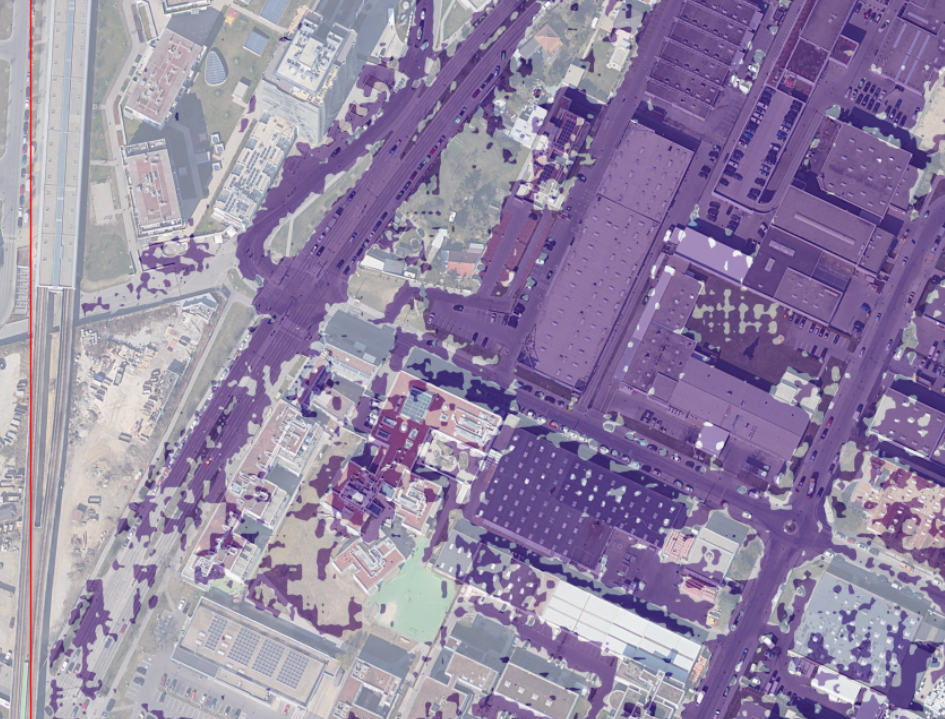
\includegraphics[width=5cm,height=3cm]{figures/fig_SAM_public_parking_space.png}}
    \end{tabular}
    \caption{The SAM model is able to fulfil only more general and common tasks.}
    \label{fig:SAM}
\end{figure}

A second version of SAM was recently released (SAM2) with viedo processing capabilities and specific code for fine tuning. Fine tuning in the context of computer vision involves taking 
a pre-trained model, which has been trained on a general and diverse 
dataset and freezing the weights of the pre-trained 
model's encoder and train a new decoder. The underlying assumption 
is that a general understanding of image patterns and features is 
transferable, independent of the specific dataset chosen, no matter 
how different the datasets might be 
\footcite{zhuang_comprehensive_2021}. However, it's 
important to note that this assumption has been empirically proven for years but the mathematical background is still under development \footcite{cao_feasibility_2023}. Fine-tuning can be applied to traditional vision models such as Mask2Former \footcite{cheng_masked-attention_2022} or to the SAM model. To fine tune the SAM model not only ground truth data is needed but user prompts have to be generated, usually by sampling random points inside the instance geometry of the ground truth.

\subsection{Instance segmentation}
\label{sec:instance_seg_bg}

The building footprint can be obtained using instance and semantic segmentation techniques. Semantic segmentation identifies, at the pixel level, whether a given pixel in an image belongs to a building or not. Instance segmentation, on the other hand, assigns a unique identifier (ID) to each segmented building, thus generating both a semantic layer and a layer with the building ID for each pixel (fig. \ref{fig:instances}). This facilitates distinguishing between different and adjacent buildings and accurately defining the boundary between them. Instance segmentation involves detecting and delineating individual objects within an image, assigning each pixel not only a class label but also a unique instance ID. Unlike semantic segmentation, which classifies pixels without distinguishing between separate instances of the same class, instance segmentation produces object-aware outputs that are better suited for generating vector geometries, making it particularly relevant for tasks like building footprint extraction in areas with touching structures. The SAM and Mask2Former models used for experiments in this study are available for semantic and instance segmentation tasks.

\begin{figure}[H]
    \centering
    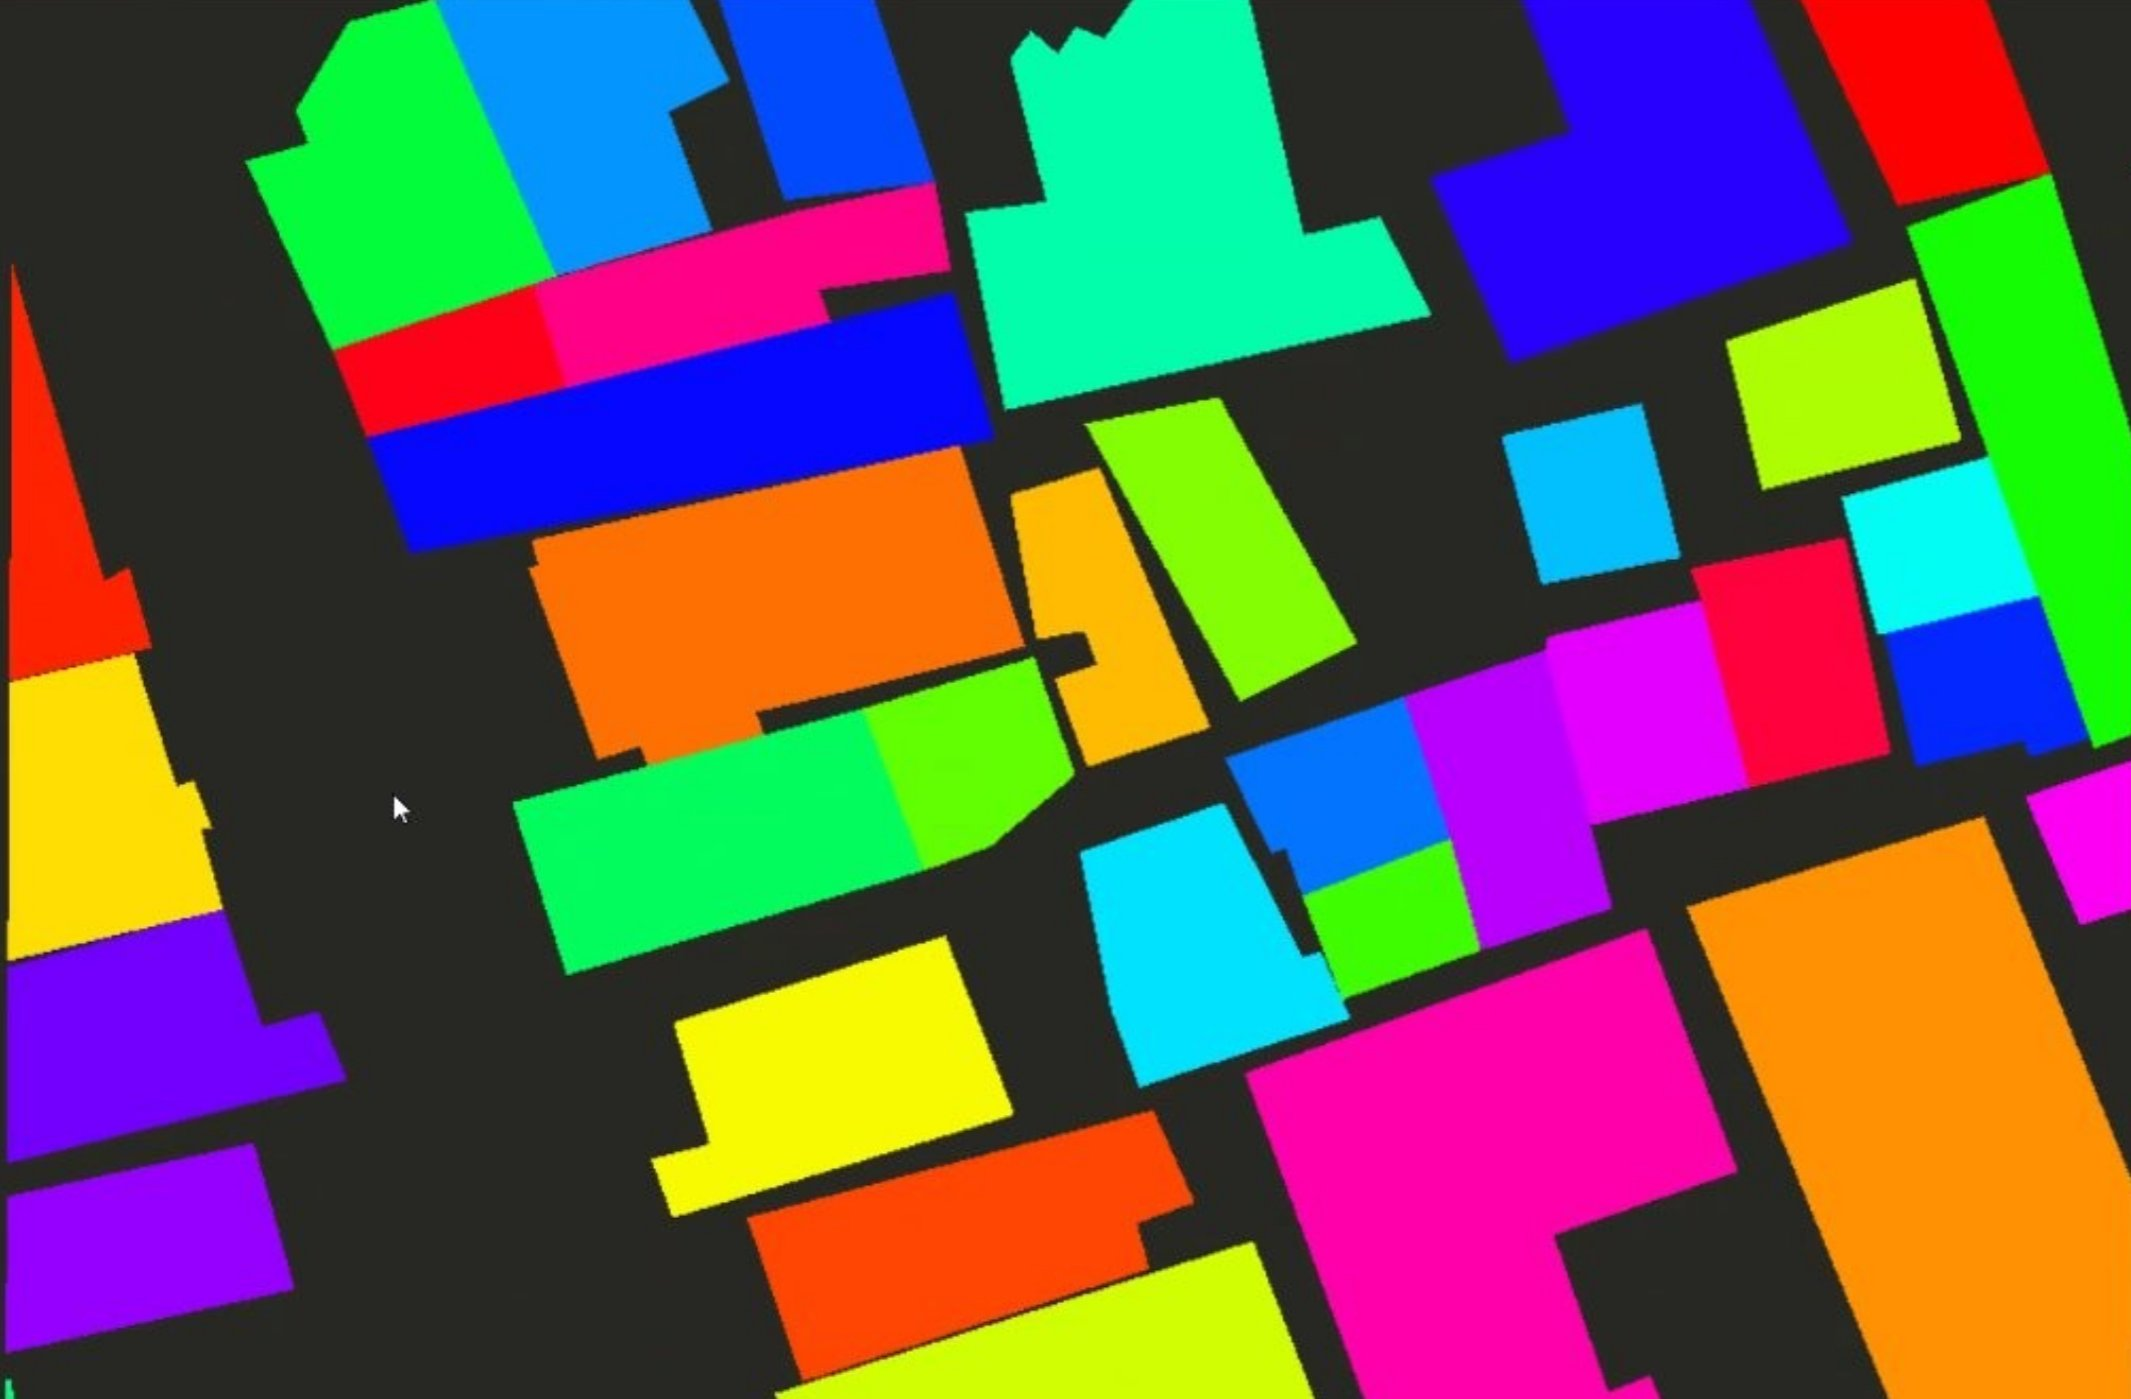
\includegraphics[width=5cm]{figures_and_references/EELISA_conference/figures/instance_segmentation.jpg}
    \caption{Example dataset with building instance ids.}
    \label{fig:instances}
\end{figure}


\newpage

\renewcommand{\sectionnametext}{References}
\renewcommand{\headingtextR}{\thesection. \sectionnametext}
\section{\sectionnametext}
\printbibliography[heading=none]

\end{refsection}